%%
% Please see https://bitbucket.org/rivanvx/beamer/wiki/Home for obtaining beamer.
%%
\documentclass[handout]{beamer}
%\usetheme{Warsaw}

\usepackage{blkarray}
\usepackage{bigstrut}
\usepackage{amsmath}
\usepackage{bbm}
\usepackage{harpoon}
\usepackage{caption}
\usepackage{subcaption}
\usefonttheme[onlymath]{serif}

\makeatletter
\let\BA@quicktrue\BA@quickfalse
\makeatother

\renewcommand{\vec}[1]{ {\bf #1} }
\newcommand{\abs}[1]{ \left\lvert #1 \right\rvert }

\title{A Supervised Learning Approach to Predicting Multigrid Convergence}
\author[me]{Nicolas Nytko\\[3mm]Matthew West, Luke Olson, Scott MacLachlan}
\date{\today}

\begin{document}
\frame{\titlepage}


% Overview
\begin{frame}
  \frametitle{Overview}
\end{frame}


% Poisson intro
\begin{frame}
  \frametitle{Poisson Problem}
  \begin{itemize}
  \item Look at the 1D variable coefficients case w/ homogeneous Dirichlet conditions
    \[ -\nabla \cdot \left(k\left(\vec{x}\right) \nabla \vec{y} \right) = f \]
    \[ \Omega = \left[-1, 1\right] \quad \partial\Omega = 0 \]
  \item Discretized on $N=31$ internal points using finite differences, $k\left(\vec{x}\right)$ is discretized on midpoints to preserve symmetry.
  \item For arbitrary C/F splitting, can we predict convergence rate and optimal relaxation weight?
  \end{itemize}
\end{frame}


\begin{frame}
  \frametitle{Training Dataset}
  \begin{itemize}
  \item For ``traditional'' machine learning we need a dataset.
    \pause
  \item Idea: Run a \textit{whole lot} of multigrid iterations.
    \pause
  \item Run multigrid iterations and record convergence rate and relaxation weight for randomly generated C/F splittings and problem setups.
  \end{itemize}
  \begin{center}
    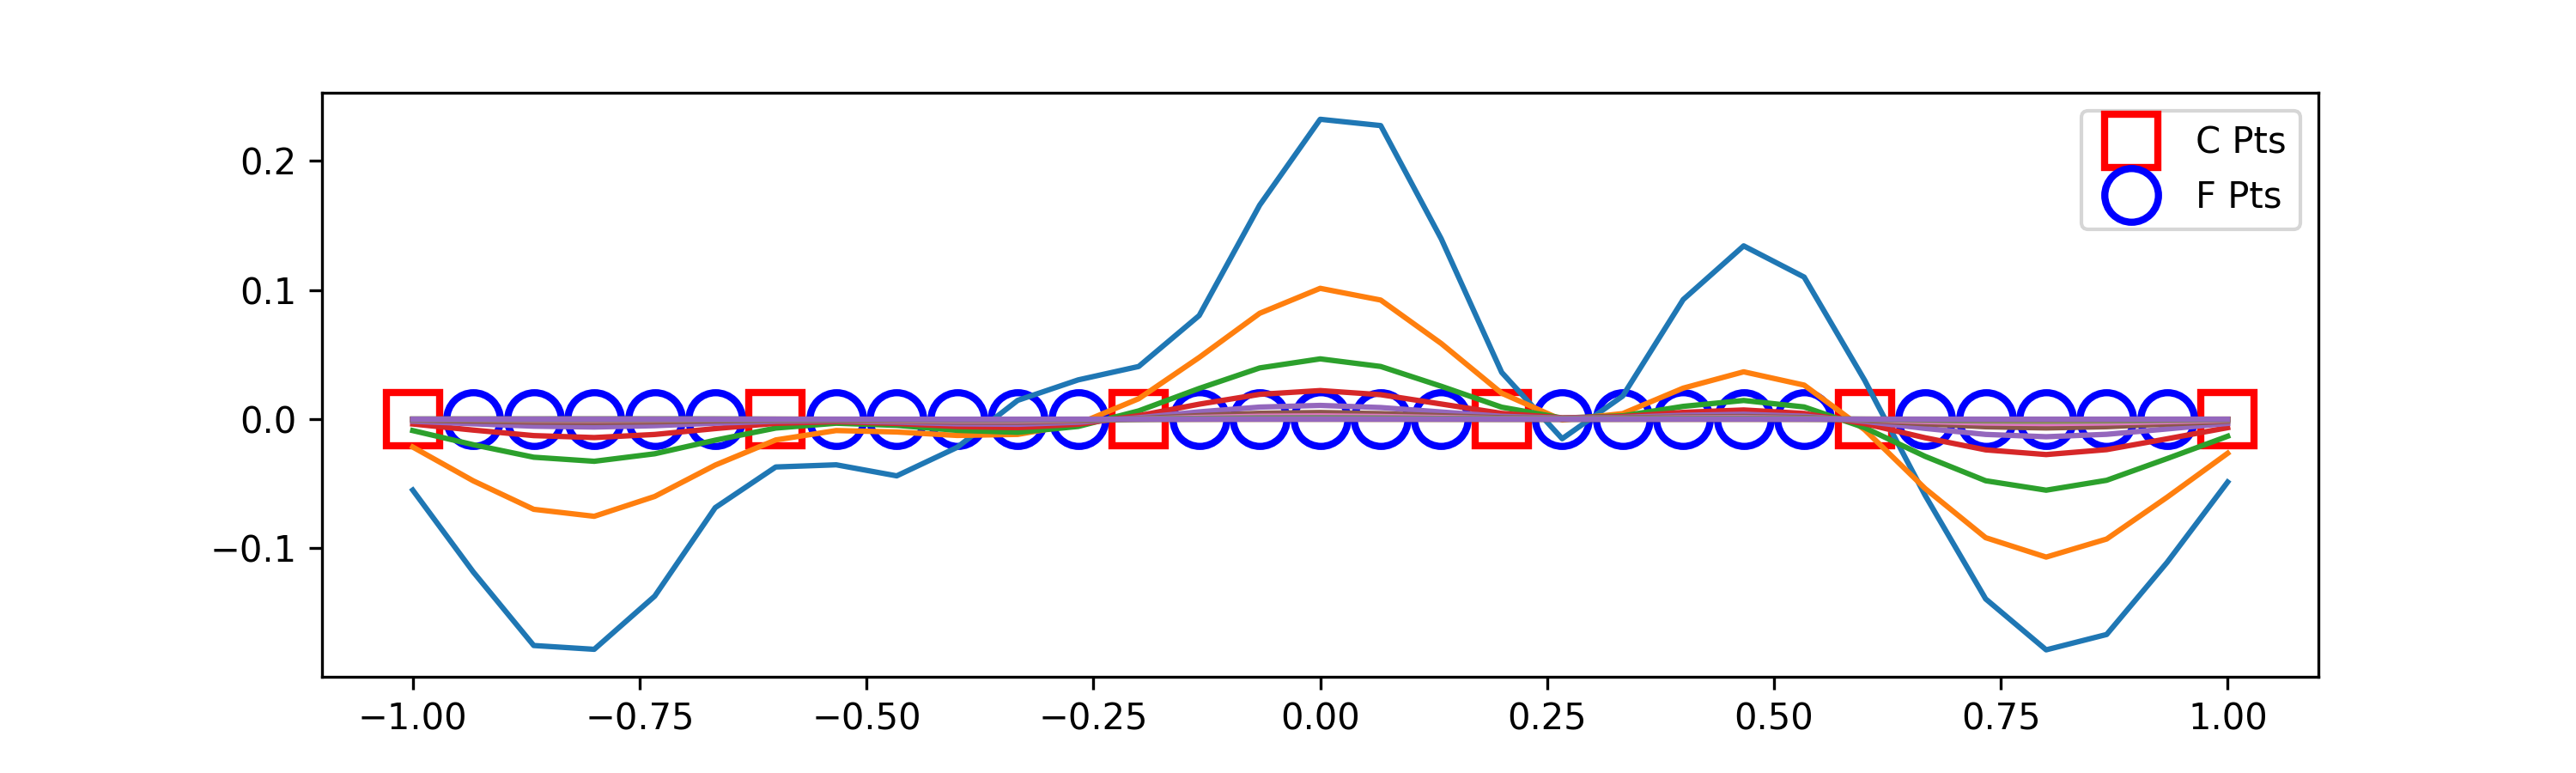
\includegraphics[width=0.8\textwidth]{figures/multigrid.png}
  \end{center}
\end{frame}


\begin{frame}
  \frametitle{Dataset Generation}
  \begin{itemize}
  \item Start from ``reference'' splittings, which are evenly spaced coarse points on a grid.
  \item Randomly perturb each reference in several trials, according to \[ p = \left\{ 0.01 \quad 0.05 \quad 0.1 \quad 0.25 \quad 0.5 \quad 0.75 \right\}. \]
  \item Generate variable coefficients such that \[ k\left(\vec{x}\right) = \begin{cases}
\alpha \\
\text{rand()}\left(\alpha + 1\right) \\
\alpha\cos\left(\pi x \beta\right) + \gamma \\
\abs{\sum_{i=1}^5 \alpha_i x^i} + 0.01
\end{cases}. \]
  \end{itemize}
\end{frame}


\begin{frame}
  \frametitle{Convolutional Network}
  \begin{itemize}
  \item Take the C/F splittings, run in multigrid solver to find convergence rate and relaxation weight that maximizes the former.
  \item Use the data to train a \textit{1D convolutional network} that predicts convergence, Jacobi relaxation.
  \end{itemize}

  \begin{table}[t]
\centering
\begin{tabular}{|l|l|l|l|}
\hline
Model & Dataset & Value \\

\hline
Jacobi Weight & Training & $1.8331 \times 10^{-3}$ \\
Jacobi Weight &  Testing & $1.8396 \times 10^{-3}$ \\
\hline
Convergence Factor & Training & $1.4839 \times 10^{-3}$ \\
Convergence Factor & Testing & $1.5171 \times 10^{-3}$ \\
\hline
\end{tabular}
\caption{Mean squared error (MSE) between predicted and true Jacobi weight, convergence factor.}
\label{tab:poisson_loss}
\end{table}
\end{frame}


\begin{frame}
  \frametitle{CNN Performance}
  \begin{figure}[h]
  \centering
  \begin{subfigure}{.48\textwidth}
    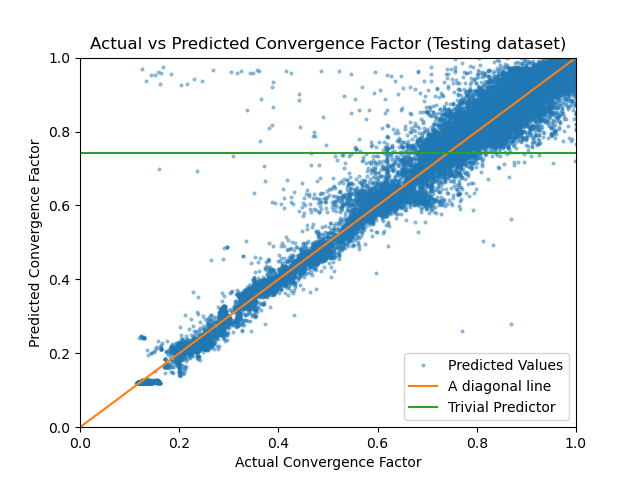
\includegraphics[width=\textwidth]{figures/poisson_conv_test_pred.png}
    \caption{Testing predictions}
  \end{subfigure}
  \begin{subfigure}{.48\textwidth}
    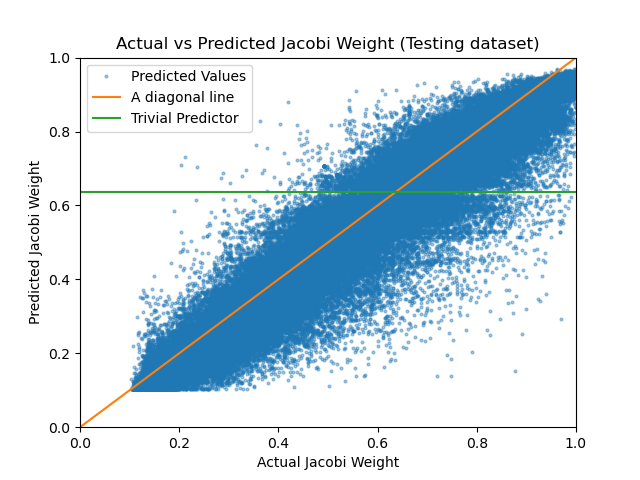
\includegraphics[width=\textwidth]{figures/poisson_jacobi_test_pred.png}
    \caption{Training predictions}
  \end{subfigure}
  \caption{(a) Predicted convergence values vs. true convergence values, (b) Predicted relaxation weights vs true relaxation weights.  Values closer to the diagonal represent more accurate predictions. }
  \label{fig:poisson_conv_pred}
\end{figure}
\end{frame}


\begin{frame}
  What we learned: \pause Poisson is too easy!
  \newline\newline
  \pause

  Let's try learning a more difficult problem.
\end{frame}


\begin{frame}
  \frametitle{Convection-Diffusion Problem}
  Try out a specific convection-diffusion problem,
  \[\vec{w}\cdot\nabla u -k\nabla^2u = f,\]
  on 2D square, $\Omega = \left[-1,1\right]^2$, discretized as quadrilateral finite elements.  Use  $k=0.1$, $\vec{w} = \begin{bmatrix} 2y(1-x^2) & 2x(1-y^2)  \end{bmatrix}$.
\end{frame}


\begin{frame}
  \frametitle{Dataset Generation, Convection-Diffusion}
  \begin{itemize}
  \item Discretize on a $25 \times 25$ structured grid.
  \item Start from ``reference'' splittings, all fine, all coarse, AMG output, etc.
  \item Randomly perturb each reference in several trials, according to \[ p = \left\{ 0.01 \quad 0.05 \quad 0.1 \quad 0.25 \quad 0.5 \quad 0.75 \right\}. \]
  \item Don't generate coefficient values for now.
  \item Take output and run through 50 iteration multigrid solver to find convergence rate.
  \end{itemize}
\end{frame}


\begin{frame}
  \frametitle{Convection-Diffusion Convolution}
  \begin{itemize}
    \item 2D structured grid $\Rightarrow$ train 2D convolutional network to predict convergence.
  \end{itemize}
\end{frame}


\begin{frame}
  \begin{itemize}
  \item Classical convolution techniques work okay on structured, grid-like inputs.
  \item Very restrictive in terms of mesh data we can use for FEM solvers.
  \item Take a look at some network architectures that allow for unstructured data: introduce \textit{graph-nets}.
  \end{itemize}
\end{frame}


\end{document}
